\documentclass[11pt,a4paper]{article}
\usepackage[margin=1in]{geometry}
\usepackage{graphicx}
\usepackage{subcaption}
\usepackage{booktabs}
\usepackage{fancyhdr}
\usepackage{enumitem}

\pagestyle{fancy}
\fancyhf{}
\lhead{Laboratory Report}
\rhead{AI5707: PRML -- Lab Assignment 6}
\cfoot{Page \thepage}
\renewcommand{\headrulewidth}{0.4pt}

\setlist[itemize]{itemsep=2pt,topsep=3pt}
\setlist[enumerate]{itemsep=2pt,topsep=3pt}

\begin{document}

\begin{center}
{\LARGE \textbf{2D Gaussian Mixture Models, K-Means Clustering, and Classification}}\\[6pt]
{\large Lab Assignment 6 Report}\\[6pt]
Shrawanthi P. (Roll No: 26120098)\\
Shreepriyadarshini RM. (Roll No: 26120099)\\[4pt]
16th October 2026
\end{center}

\section{Objective}
The main goals of this assignment are:
\begin{enumerate}
  \item Generate 2D synthetic data for two distinct classes using Gaussian Mixture Models (GMMs) with $K=3$ components per class.
  \item Experiment with three different covariance types across the components: isotropic ($\sigma^2 \mathbf{I}$), diagonal, and full covariance matrices.
  \item Visualize the generated data points with different colors for each cluster.
  \item Split the dataset of each class into an 80\% training set and a 20\% test set.
  \item Perform K-Means clustering on the 80\% training data to discover cluster centers and plot cluster boundaries.
  \item Classify the 20\% test data using the learned cluster centers based on minimum distortion (distance to the nearest cluster center).
  \item Evaluate classification performance with a confusion matrix and plot the resulting decision boundary.
\end{enumerate}

\section{Workflow}
The experiment is executed in four straightforward steps:
\begin{enumerate}
  \item \textbf{Data Generation:}
  We generate 4,000 2D points for Class 1 and 4,000 points for Class 2 (8,000 points in total). Each class consists of three Gaussian components with assigned weights, centers, and covariance shapes (isotropic, diagonal, and full). Points are drawn using standard normal random numbers transformed by the mean and covariance of each component.
  
  \item \textbf{Train-Test Split:}
  Each class is randomly shuffled and divided into:
  \begin{itemize}
    \item \textbf{Training set (80\%):} 3,200 points per class (used for clustering).
    \item \textbf{Test set (20\%):} 800 points per class (used for classification evaluation).
  \end{itemize}

  \item \textbf{K-Means Clustering on Training Data:}
  K-Means ($K=3$) is run separately on the training data of Class 1 and Class 2. The algorithm automatically locates the three cluster centers for each class without any class or component labels. Multiple random starts are used to ensure optimal convergence.

  \item \textbf{Classification via Minimum Distortion:}
  For each test sample, we measure its squared Euclidean distance to the nearest cluster center of Class 1 and to the nearest cluster center of Class 2. The sample is assigned to the class that gives the smaller distance (minimum distortion).
\end{enumerate}

\section{Outputs and Results}

\subsection{Parameters Used for Data Generation}
Table~\ref{tab:params} lists the chosen mixing weights, centers, and covariance matrices for the two classes.

\begin{table}[ht]
\centering
\small
\begin{tabular}{@{}lcccc@{}}
\toprule
\textbf{Class \& Component} & \textbf{Covariance Type} & \textbf{Weight} & \textbf{True Center ($\mu$)} & \textbf{Covariance Matrix ($C$)} \\
\midrule
Class 1, Component 0 & Isotropic & 0.30 & $[-9.0, 7.0]^T$ & $\begin{bmatrix} 1.0 & 0.0 \\ 0.0 & 1.0 \end{bmatrix}$ \\[5pt]
Class 1, Component 1 & Diagonal  & 0.45 & $[-9.0, 0.0]^T$ & $\begin{bmatrix} 0.5 & 0.0 \\ 0.0 & 2.0 \end{bmatrix}$ \\[5pt]
Class 1, Component 2 & Full      & 0.25 & $[-9.0, -7.0]^T$ & $\begin{bmatrix} 2.0 & 0.8 \\ 0.8 & 1.0 \end{bmatrix}$ \\
\midrule
Class 2, Component 0 & Isotropic & 0.35 & $[-1.0, 7.0]^T$ & $\begin{bmatrix} 1.0 & 0.0 \\ 0.0 & 1.0 \end{bmatrix}$ \\[5pt]
Class 2, Component 1 & Diagonal  & 0.25 & $[-1.0, 0.0]^T$ & $\begin{bmatrix} 1.5 & 0.0 \\ 0.0 & 0.7 \end{bmatrix}$ \\[5pt]
Class 2, Component 2 & Full      & 0.40 & $[-1.0, -7.0]^T$ & $\begin{bmatrix} 1.5 & -0.6 \\ -0.6 & 1.0 \end{bmatrix}$ \\
\bottomrule
\end{tabular}
\caption{Parameters for Class 1 and Class 2 components.}
\label{tab:params}
\end{table}

\subsection{GMM Data Plot}
Figure~\ref{fig:gmm} displays the generated points for both classes. Each component is plotted in a different color to highlight its distinct shape.

\begin{figure}[ht]
\centering
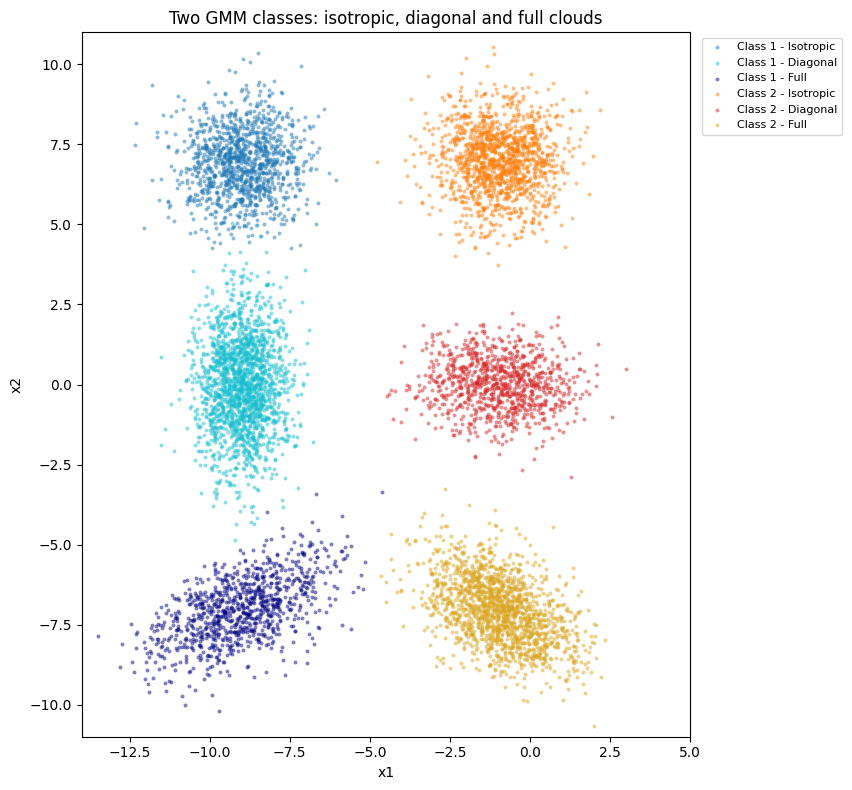
\includegraphics[width=0.72\textwidth]{Gmm_of_both_classes.png}
\caption{Generated 2D data for Class 1 (left) and Class 2 (right) across isotropic, diagonal, and full covariance components.}
\label{fig:gmm}
\end{figure}

\subsection{K-Means Clustering Outputs}
Table~\ref{tab:centers} compares the original true means with the centers discovered by K-Means on the training data. Figure~\ref{fig:kmeans} shows the learned cluster boundaries and centers.

\begin{table}[ht]
\centering
\small
\begin{tabular}{@{}lccc@{}}
\toprule
\textbf{Class \& Component} & \textbf{True Center} & \textbf{K-Means Discovered Center} & \textbf{Difference} \\
\midrule
Class 1, Top (Isotropic)    & $[-9.00, \phantom{-}7.00]^T$ & $[-9.01, \phantom{-}6.90]^T$ & $[0.01, 0.10]^T$ \\
Class 1, Middle (Diagonal)  & $[-9.00, \phantom{-}0.00]^T$ & $[-9.00, -0.04]^T$           & $[0.00, 0.04]^T$ \\
Class 1, Bottom (Full)      & $[-9.00, -7.00]^T$           & $[-9.06, -7.02]^T$           & $[0.06, 0.02]^T$ \\
\midrule
Class 2, Top (Isotropic)    & $[-1.00, \phantom{-}7.00]^T$ & $[-0.97, \phantom{-}7.00]^T$ & $[0.03, 0.00]^T$ \\
Class 2, Middle (Diagonal)  & $[-1.00, \phantom{-}0.00]^T$ & $[-0.96, \phantom{-}0.02]^T$ & $[0.04, 0.02]^T$ \\
Class 2, Bottom (Full)      & $[-1.00, -7.00]^T$           & $[-0.94, -7.07]^T$           & $[0.06, 0.07]^T$ \\
\bottomrule
\end{tabular}
\caption{True means versus learned K-Means cluster centers.}
\label{tab:centers}
\end{table}

\begin{figure}[ht]
\centering
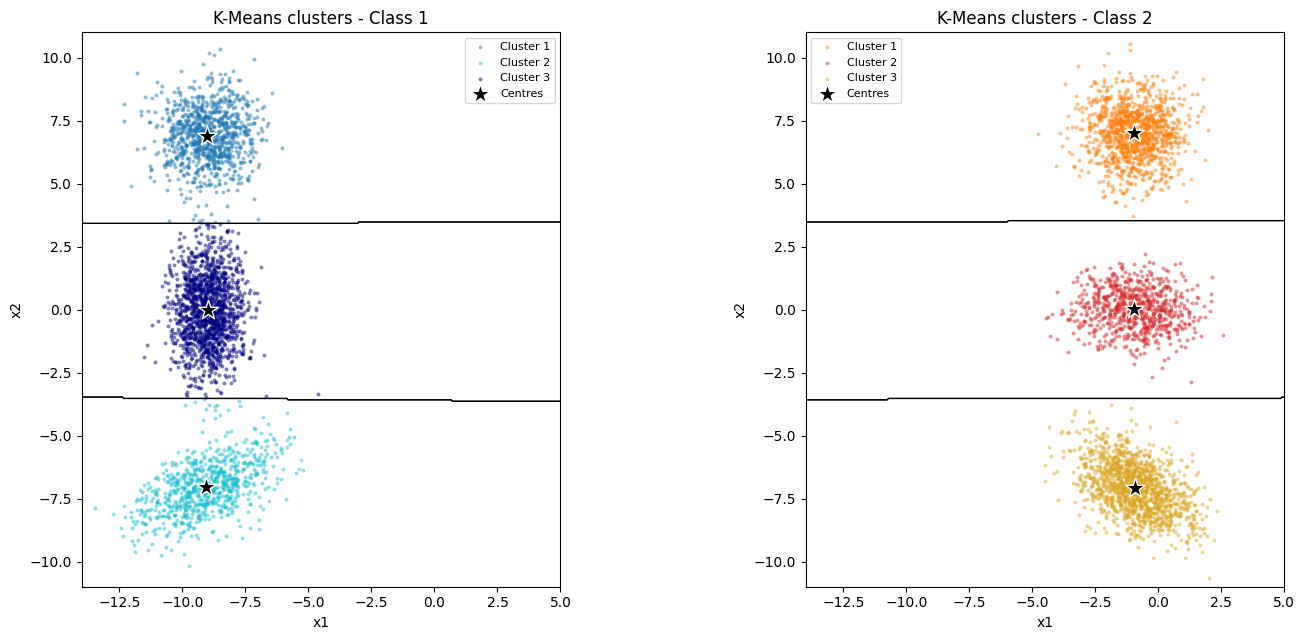
\includegraphics[width=0.98\textwidth]{k_means_clustering.png}
\caption{K-Means cluster assignments, centers (stars), and intra-class boundaries for Class 1 (left) and Class 2 (right).}
\label{fig:kmeans}
\end{figure}

\subsection{Classification Results and Decision Boundary}
Using the learned cluster centers, the 1,600 test samples were classified by minimum distortion. Table~\ref{tab:confusion} presents the confusion matrix, and Figure~\ref{fig:decision} shows the resulting decision boundary.

\begin{table}[ht]
\centering
\begin{tabular}{lcc}
\toprule
\textbf{True Class} & \textbf{Predicted Class 1} & \textbf{Predicted Class 2} \\
\midrule
\textbf{Class 1} & 800 & 0 \\
\textbf{Class 2} & 0 & 800 \\
\bottomrule
\end{tabular}
\caption{Confusion matrix on 1,600 test points (Test Accuracy: 100.0\%).}
\label{tab:confusion}
\end{table}

\begin{figure}[ht]
\centering
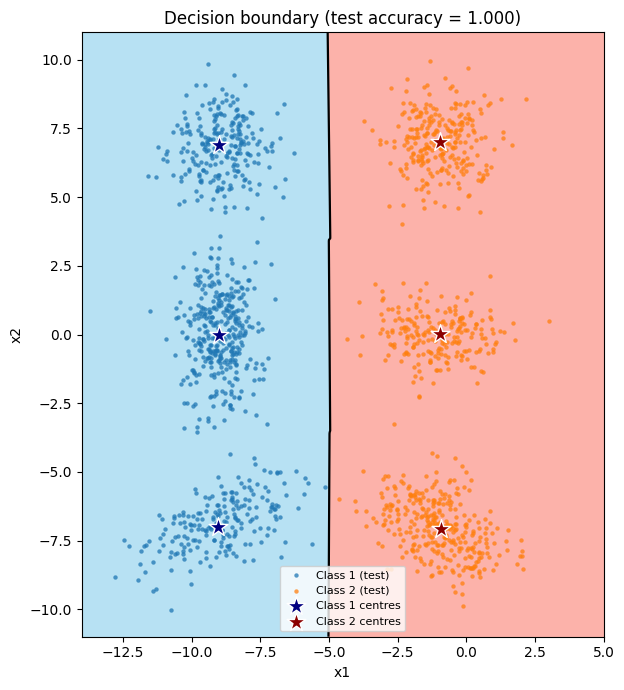
\includegraphics[width=0.68\textwidth]{decision_boundary.png}
\caption{Decision regions (blue for Class 1, red for Class 2) and decision boundary at $x_1 \approx -5.0$ overlaid with test points and cluster centers.}
\label{fig:decision}
\end{figure}

\section{Findings}
\begin{itemize}
  \item \textbf{Shape of Covariance Clouds:}
  \begin{itemize}
    \item \textit{Isotropic:} Equal spread in all directions produces circular clusters.
    \item \textit{Diagonal:} Unequal variances along coordinate axes produce axis-aligned elliptical clusters (Class 1 is stretched vertically; Class 2 is stretched horizontally).
    \item \textit{Full Covariance:} Off-diagonal terms tilt the distribution diagonally (Class 1 tilts upward with positive correlation; Class 2 tilts downward with negative correlation).
  \end{itemize}

  \item \textbf{Clustering Accuracy:}
  K-Means successfully discovered all component centers without supervision. The discovered centers closely match the true parameters with an error of less than $0.1$ units.

  \item \textbf{Decision Boundary Behavior:}
  Because Class 1 centers are centered at $x_1 \approx -9.0$ and Class 2 centers are centered at $x_1 \approx -1.0$, the minimum distortion rule forms a vertical decision boundary at $x_1 \approx -5.0$ (midway between the two classes).

  \item \textbf{Classification Performance:}
  Both classes are cleanly separated, yielding zero test errors and a test accuracy of $100.0\%$ ($1,600 / 1,600$ correct).
\end{itemize}

\end{document}
